\documentclass[12pt,letterpaper]{article}

\title{The Steiner Tree Problem (1991)}
\author{Peter Gordon \and Casey Cao-Son \and Brennan Truong}
\date{December 12, 2014}

\usepackage{amsmath}
\usepackage{amsfonts}
\usepackage{amssymb}
\usepackage{amsthm}
\usepackage[top=.5in,bottom=.5in,left=1in,right=1in]{geometry}
\usepackage{tikz}
\usepackage[pdftitle={The Steiner Tree Problem (1991)},
	pdfauthor={Peter Gordon, Casey Cao-Son, Brennan Truong},
	pdfsubject={MATH 370}]{hyperref}
\usepackage{float}

%\linespread{1.6} %% "double" space text

\newcounter{defncounter}
\theoremstyle{definition}\newtheorem{defn}[defncounter]{Definition}

\theoremstyle{remark}\newtheorem*{remark}{Remark}

\newcommand{\HRule}{\rule{\linewidth}{0.5mm}}

\begin{document}
\begin{titlepage}
\begin{center}

% Upper part of the page. The '~' is needed because \\
% only works if a paragraph has started.

\includegraphics[width=0.45\textwidth]{CSUFLogo}~\\[1cm]


\textsc{\Large Math 370 Semester Project}\\[0.5cm]

% Title
\HRule \\[0.4cm]
{ \huge \bfseries The Steiner Tree Problem (1991) \\[0.4cm] }

\HRule \\[1.5cm]

% Author and supervisor
\noindent
\begin{minipage}[t]{0.4\textwidth}
\begin{flushright} \large
\emph{Authors:}\\
Peter \textsc{Gordon} \\
Casey \textsc{Cao-Son} \\
Brennan \textsc{Truong}
\end{flushright}
\end{minipage}
\hfill
\begin{minipage}[t]{0.4\textwidth}
\begin{flushleft} \large
\emph{Professor:} \\
Dr.~Laura \textsc{Smith}
\end{flushleft}
\end{minipage}
\vfill

% Bottom of the page
{\large December 12, 2014}

\end{center}
\end{titlepage}


\section{Introduction}
The infrastructure of most modern communication is a wired network. Stations, terminals, and devices are connected through a 
network of cables and wires to transmit information. It is easy to see that the cost of these cables is proportional to their 
length: a longer cable requires more data wiring, insulation, and so on. So how do we ensure that cost is minimized? Not only 
this, but any extraneous cabling would also increase the latency (propogation delay) in the network, making it slower for its 
users. Because of these, among other reasons, we want to optimize the network to minimize the total wiring. In addition,
similar optimizations are beneficial in other fields, such as VLSI (Very Large Scale Integrated Circuits) layouts.

We can use graph theory to help analyze and optimize this network. First, this wired network can be thought of as a connected 
weighted graph, with each node (terminal or device) being a vertex, the connections being the set of edges, and the the cost of 
the cable between them being the weights of those edges. As a natural consequence of analyzing the network through graph theory, 
it would seem that the optimal way to create the network would be according to the minimum spanning tree of the representative 
graph.

Indeed, this is ideal without any modifications to the graph; but in the Steiner Tree Problem, extra intermediary points (called 
\emph{Steiner points}) are added to the graph to reduce the total weight of edges between groups of points, and thereby reduce the 
total spanning tree weight. Therefore, the Steiner Tree Problem is superficially similar to that of finding the minimum spanning 
tree, but with the added benefit (and complexity) of introducing other vertices where needed.

\section{Problem Statement}

Using rectilinear (sometimes called ``taxicab'') distances, we are to create a minimal-cost spanning tree (e.g, Steiner Tree) for a 
network with nine stations: \[a(0, 15), \quad b(5, 20), \quad c(16, 24), \quad d(20, 20), \quad e(33, 25) \] \[ f(23, 11), \quad 
g(35, 7), \quad h(25, 0), \quad i(10, 3) \text{.}\] Any added phantom stations (Steiner points) must be integer coordinates. The cost 
(weight) of each line is its length.

A second problem adds to this a per-station cost of \(d^{3/2}w\), where \(w = 1.2\) and \(d\) is the degree of that station (i.e., 
the number of edges it has). We are then to calculate a new minimal-cost spanning tree with these costs.

Lastly, we are to generalize the problem.


\section{Literature Review}

Upon searching related literature, we discovered Dr. A. Greenbaum's lecture notes for Math 381 (Discrete 
Mathematical Models) at the University of Washington. In this lecture, Dr. Greenbaum presents an excellent summary of many 
algorithms such as Prim's algorithm to find the minimal spanning tree of a graph. This will be useful as a final step in 
construction of the minimal Steiner tree. 

However, the first step is to find the possible Steiner points (or ``phantom stations'' as they are deemed in this project). Maurice 
Hanan (1966) proved that the Hanan grid for a set of points must contain a minimimal rectilinear Steiner tree for those points, 
with possible Steiner points at other intersection points on this grid. Hanan's theorem is particularly useful to our work becaue 
it not only guarantees that a solution exists, but it also gives rise a possible method of constructing that solution.

In this project, we will construct the minimal Steiner tree using a similar manner. Dreyer and Overton (1998) presented two 
heuristics, the Steiner Insertion heuristic and the Incremental Optimization heuristic, to find the minimal Steiner tree using 
Euclidean (rectilinear) length. Both methods used several algorithmic tools such as the Local Optimization Algorithm, the Exact Steiner 
Algorithm, and construction of a minimal spanning tree.


\section{Assumptions}

For the reason that it is given in the problem statement, the first assumption made in this project is that all distances are 
rectilinear, rather than their usual Euclidean metric. For example, for the purposes of this project, the distance between \((0, 
0)\) and \((3, 4)\) is 7, not 5. Secondly, as this model is for a communication network, we assume for simplicity of calculations, that
\begin{enumerate}
\item[(1)] { cabling can be laid with no interference from obstacles or obstructions, such as impassable terrain or pre-existing
structures; }
\item[(2)] { the cost of the cabling is uniform, regardless of its type (such as ethernet, copper coaxial, or fiber optic); and }
\item[(3)] { cables can only be laid in straight horizontal and vertical lines. (That is, any change in direction would need an intermediary Steiner point.) }
\end{enumerate} 

\section{Solution}
Our project will design, implement, and verify an algorithm for determining the necessary Steiner points and 
finding the total minimal rectilinear Steiner tree of a given weighted graph. We approach this by two methods. 

\subsection{Hanan/Prim Hybridization} 
The first is a simple hybridization approach.  The construction of this minimal Steiner tree 
will consist of multiple steps. To begin, the Hanan Grid for the set of points is generated. By Hanan's theorem, this grid must 
contain the minimal Steiner tree to be found. This grid is a complete connected weighted graph, whose vertices are all 
intersections of the grid and whose edges have weights equal to their distances. Next, remove all vertices in the Hanan grid with 
order 1 or 2 that are not adjacent to a starting vertex. Repeat this step as needed on the graph until all vertices have order 3 
or 4. Then, to this new graph we apply Prim's algorithm to determine the minimum spanning tree including the Steiner points. When 
finished, the graph is complete in that it includes all of the starting points as well as any needed Steiner points. (Note that as 
part of the process of creating this Steiner tree, some of the points from the earlier Hanan grid are removed from the graph.)

\subsection{Modifying Prim's Algorithm}
Our second approach is to modify Prim's Algorithm so that it can be applied directly to 
the initial set of points without having to first construct the Hanan Grid (which for large sets of points can be very 
resource-intensive). In order to accomplish this, we add additional state-tracking to the algorithm by keeping a running list of 
all disconnected vertices mapped to both the distance and closest point in the growing tree to each.  Morever, when attempting to 
add that edge, if the two points are not on the same horizontal or vertical line, the Steiner point is created between them. As 
this gives two possibilities for each needed Steiner point (using the \(x\)-coordinate of one and the \(y\)-coordinate of the 
other), we further try to optimize the result by choosing the more optimal of the two: the Steiner point is chosen to lie on a 
pre-existing edge of the graph near the vertex if possible, or simply the closer point to the geometric center of the graph if 
not. This aims to minimize the total number of added Steiner points, adding them only on an as-needed basis during the tree 
construction.

These solutions were devised in order to theoretically solve \emph{any} Steiner tree problem, given an arbitrary set of starting 
points and a distance metric between two points. This gives an easy way to answer both the first and the third question. Morever, 
with the distance metric being arbitrary, it is a simple matter of adding in the \(d^\frac{3}{2}w\) weight at each point in the 
calcations to answer the second. 


\section{Solution}

\subsection{Result Graphs}
The resulting graphs for the two methods are shown.
%\begin{minipage}[]{0.45\textwidth}
 \begin{figure}[htbp!]
  	\centering
 	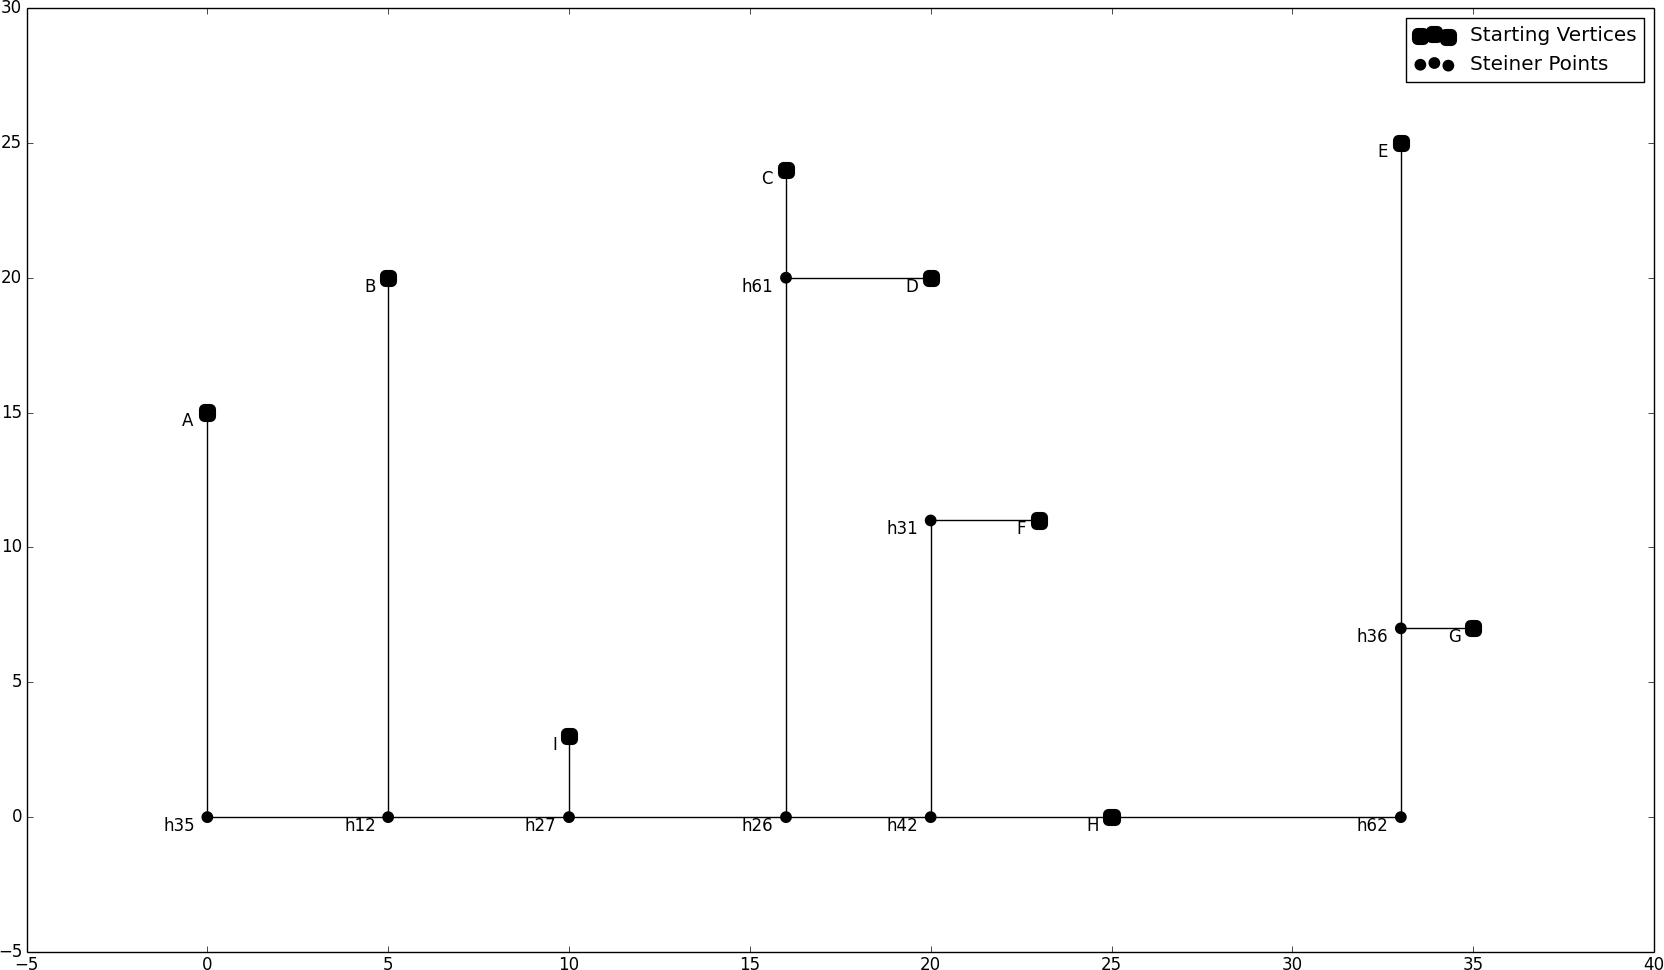
\includegraphics[width=0.6\textwidth]{NaiveResult}
  	\caption{Result MRST -- Hybridized Approach -- Total Weight: 140 \& 187.59} 
  	\label{naiveresult_image}
  	\end{figure}
% \end{minipage}

%\begin{minipage}{0.45\textwidth}
 \begin{figure}[htbp!]
  	\centering
 	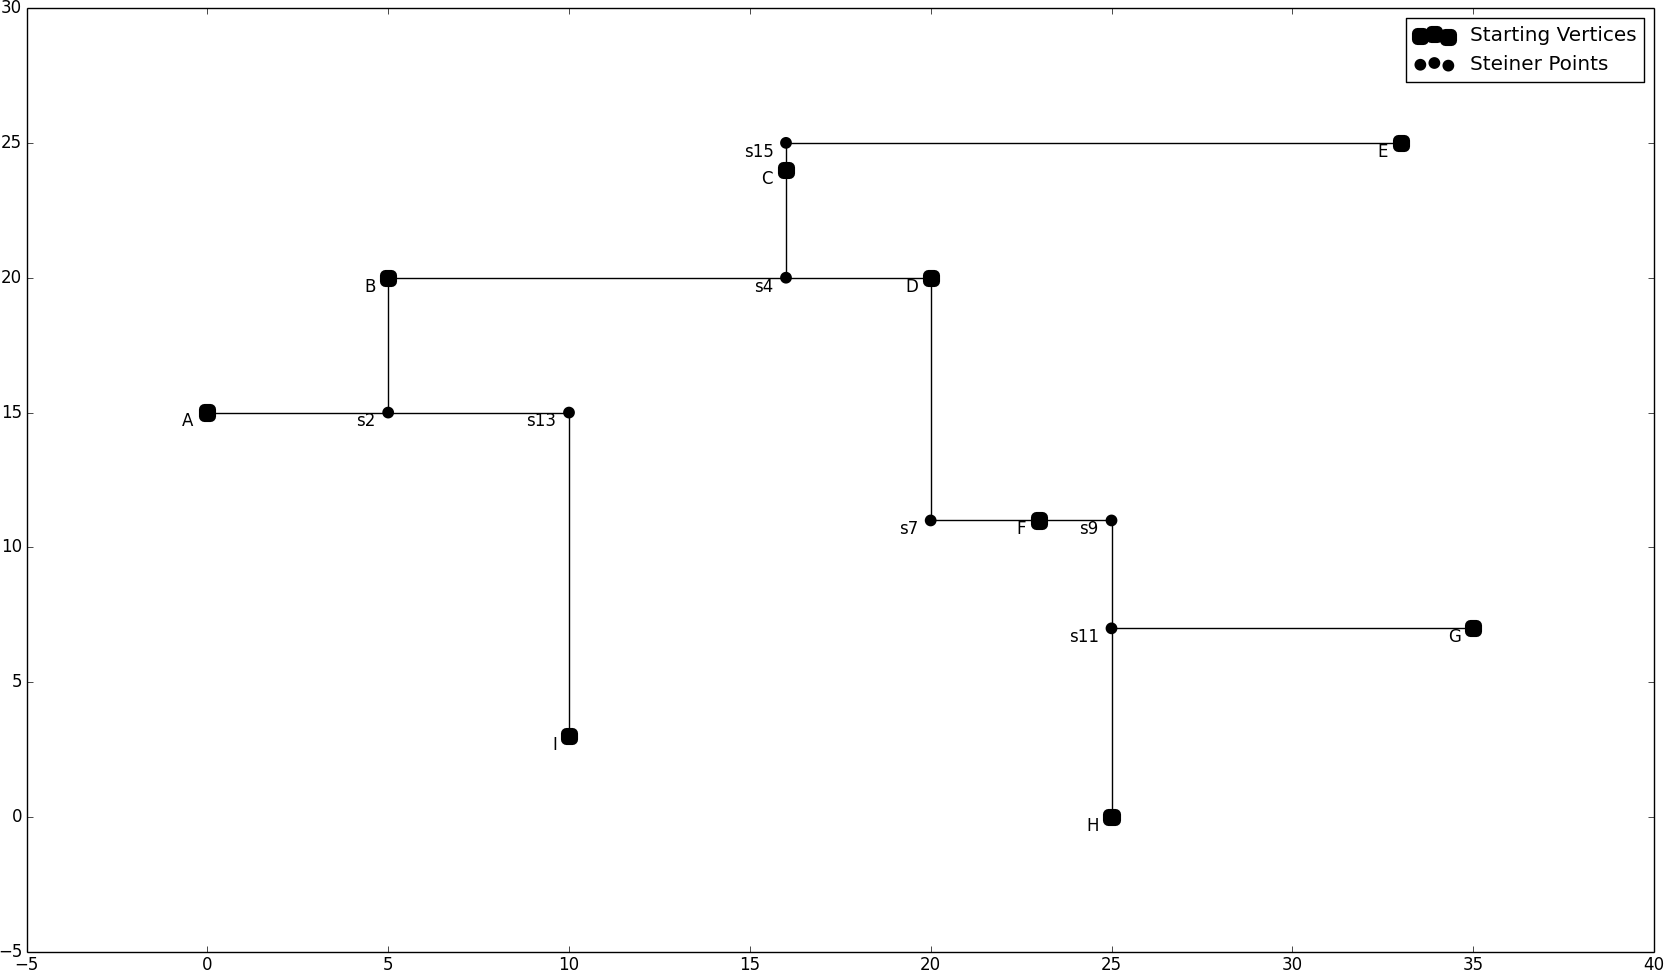
\includegraphics[width=0.6\textwidth]{SmarterResult}
  	\caption{Result MRST -- Modified Prim's Approach -- Total Weight: 140 \& 187.59} 
  	\label{smarterresult_image}
  	\end{figure}
% \end{minipage}


\subsection{Results Discussion} 
The weights with each graph shown include both with and without the \(d^{3/2}w\) weight at each station. Perhaps a bit 
counterintuitively, the Hanan/Prim hybridization approach appears to calculate a more precise minimum rectilinear Steiner tree for 
these; but this method requires construction of the entire Hanan grid, and so is a much more time- and resource-intensive 
algorithm than our modified Prim's Algorithm. Consider the worst case, in which the starting set of \(v\) points has none that lie 
on the same horizontal or vertical line, then its associated Hanan grid has \(v^2\) vertices, and as Prim's algorithm is also 
quadratic, this hybrid approach becomes one of fourth-order running time. On the other hand, it confers the advantage of simpler 
code and being deterministic.

However, this slight increase of precision comes at a great cost, as even with 50-100 vertices the hybridized algorithm is almost 
too slow to be usable, whereas the modified Prim's Algorithm only takes a few seconds to obtain its answer; and for medium- to 
larger-size sets of points, even when the hybridized method was still feasible, it produced a worse result. We attribute this to 
the local-optimization characteristic of the modified Prim's Algorithm, which is that at each decision of choosing the next 
disconnected vertex, or adding a Steiner point if necessary, the algorithm attempts to make the most optimal choice without 
affecting or being affected by the remainder of the graph. Like the original Prim's algorithm, this has second-order running time.

\section{Conclusion}

In his work, Hwang proved that the minimum spanning tree over a Hanan grid is a 1.5-approximation of the true minimum rectilinear 
Steiner tree. That is, this minimum spanning tree has a total weight no more than 1.5 times that of the true minimum rectilinear 
Steiner tree. While an exhaustive search algorithm could find the exact result in factorial time complexity, in this project have 
devised an algorithm that compares well to the desired result in only second-order running time, trading some accuracy for speed and 
computational feasibility while still having that guarantee of being sufficiently close to the true result to still be a useful answer.

However, the assumptions by which we simplified our original model were slightly unrealistic. For one, it is extremely unlikely 
that there would be no interfering structures in a well-populated urban or suburban area in which the communication network would 
be laid. Also, cabling does not have uniform costs. Ethernet is relatively inexpensive, but copper co-axial cabling (such as that 
used for modern cable internet/television servives) or high-bandwidth fiber optic cabling could be significantly more costly. 
Lastly, real cables can bend and don't need a routing station simply to change direction; although one could argue that for such 
vertices adding a full Steiner station could model adding a full routing hub to provide some future-proofing and room for the 
network to grow when the need arises (such as a surge in population).


\section{Future Work} It would be interesting to use other minimum spanning tree-generating algorithms (such as Kruskal's) in a 
similar manner, to see if they can be similarly modified and how their performance compares. Being able to model problems such as 
terrain or structures in the grid would also make the algorithm more realistic, and more applicable to real-world scenarios. As it 
currently is, such obstacles can be modeled by having the per-station weight function return \(+\infty\) (\texttt{float("inf")} in 
Python) for impassable terrain, or arbitrarily high values for areas that could still be routed through but with significantly 
more difficulty (such as having to lay cables on the bed of a large body of water).


\section{Glossary \& Definitions}

\begin{defn}[Weighted Graph]\label{graph_defn}

A \emph{weighted graph} \(G = (V, E)\) is a pair of a set of 
points (called \emph{vertices}) \(V\) and the set of \emph{edges}, \(E\), where each edge in \(E\) is a 3-tuple consisting of two 
vertices in \(V\) combined with a nonnegative real number \emph{weight}. That is, each edge is an element of the form \((v_a, v_b, 
w_{a,b})\) with \(v_a\), \(v_b \in V\) and \(w_{a,b} \in \left\{x \in \mathbb{R} \,\vert\, x > 0\right\}\). The \emph{weight of 
\(G\)} is the sum of all its edge weights.


\end{defn}

\begin{defn}[Connectedness]\label{connectedness_defn}

Given a weighted graph \(G\) = (\(V\), \(E\)), two vertices \(v_1\) and \(v_2\) in \(V\) are said to be \emph{adjacent} provided 
that there exists an edge between them. That is, they are adjacent when there exists some edge \(e \in E\) such that \(e = 
(v_1, v_2, w_{1,2})\) or \(e = (v_2, v_1, w_{1,2})\) for some weight \(w_{1,2}\).

Furthermore, any two vertices \(v_a\) and \(v_b\) are \emph{connected} provided that there exists an ordered sequence \(P\) of 
vertices \((v_{P_0} = v_a , v_{P_1}, v_{P_2}, \ldots, v_{P_{n-1}}, v_{P_n} = v_b)\) such that every sequential pair of vertices is 
adjacent. That is, \(v_a\) is adjacent to \(v_{P_1}\), \(v_{P_1}\) is adjacent to \(v_{P_2}\), and so on. \(P\) is called the 
\emph{path between} \(v_a\) and \(v_b\) (or alternatively, \(v_a\) and \(v_b\) are \emph{connected through} \(P\)).

A weighted graph is a \emph{connected graph} provided that every possible pair of its vertices is
connected.

\end{defn}


\begin{defn}[Hanan Grid]\label{hanangrid_defn}

Given a set of points, its \emph{Hanan Grid} is a grid composed of horizontal and vertical lines that intersect at all of the points.

\begin{figure}[H]
	\centering
	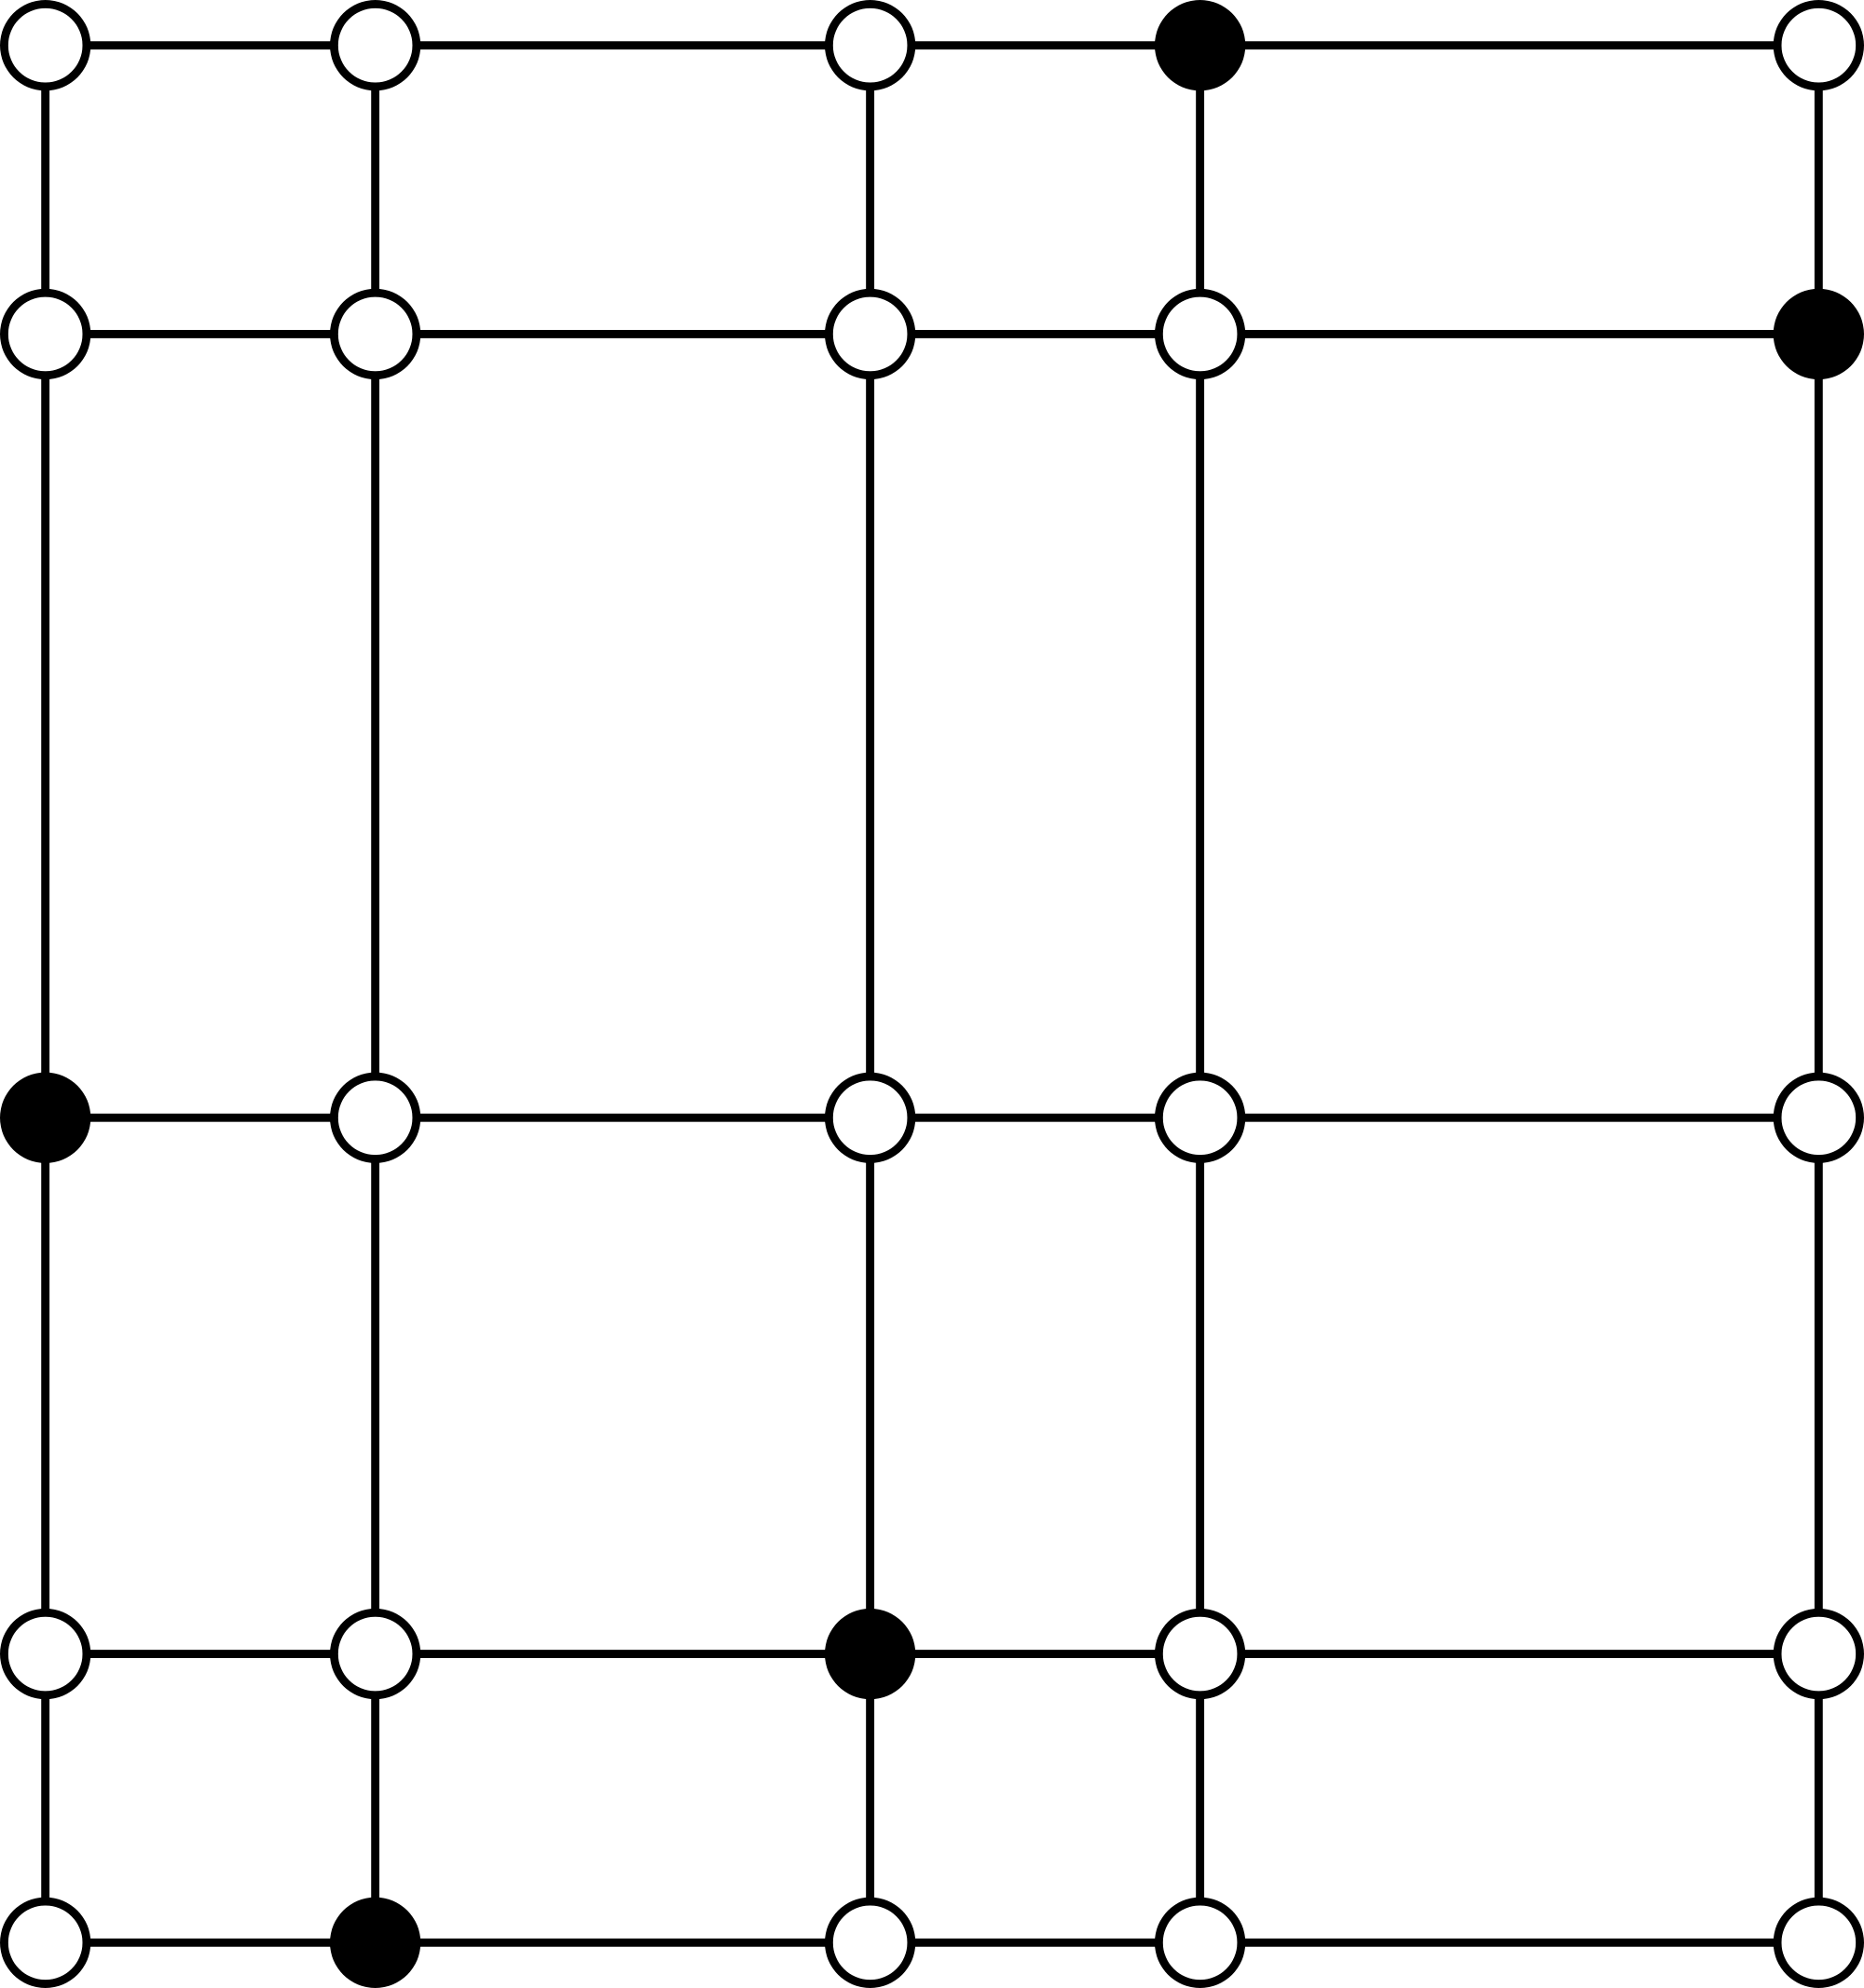
\includegraphics[width=3in]{HananGrid}
	\caption{Hanan grid generated for 5 points, by Jeffrey Sharkey, on Wikipedia.}
	\label{hanangrid_image}
\end{figure}
\end{defn}

\begin{defn}[Minimum Spanning Tree]\label{MST_defn}

Given a connected graph \(G = (E, V)\), the \emph{spanning tree} \(T\) of \(G\) is a connected graph with the same vertices as \(G\), whose edges form a subset of \(E\), and in which each pair of vertices is connected through exactly one path.

Furthermore, \(T\) is the \emph{minimum spanning tree} of \(G\) provided that the weight of \(T\) is the smallest among all
spanning trees of \(G\).

\begin{remark}

It is possible for \(G\) to have multiple different minimum spanning trees, in particular if it has many edges of the same weight; 
but; but each such minimum spanning tree would have the equal total weight.

\end{remark}

\end{defn}


\begin{defn}[Order of A Vertex]\label{vertexorder_defn}

Given a weighted graph \(G = (V, E)\), The \emph{order of a vertex} \(v\) is the number of edges which connect \(v\) to another 
vertex in \(V\).

\end{defn}


\begin{defn}[Prim's Algorithm]\label{prim_algorithm}

\emph{Prim's Algorithm} is a greedy method for finding the minimum spanning 
tree for a connected graph, consisting of three steps. 
\begin{enumerate} \item[(1)] { Initialize an empty tree with one vertex 
from the graph. } \item[(2)] { Of all the edges in the graph which connect this tree to vertices not yet in the tree, find the 
smallest-weight edge and add it to the tree. } \item[(3)] { Repeat step (2) until all vertices are in the tree. }

\end{enumerate}
\end{defn}



%% Automatically adds the \section header

\begin{thebibliography}{10}
\bibitem{DreyerOverton}
Dreyer, D., and Overton,  M. (1998). \textit{Two heuristics for the Euclidean Steiner tree problem}. Journal of Global Optimization, 13(1), 
95-106.

\bibitem{Greenbaum}
Greenbaum, A. (2006). Discrete Mathematical Model [Lecture Note]. Retrieved from 
\url{https://www.math.washington.edu/~greenbau/Math_381/notes/381notes.pdf}

\bibitem{Hanan}
Hanan, M., \textit{On Steiner's problem with rectilinear distance}. SIAM J. Applied Math., 14:255– 265, 1966.

\bibitem{Sharkey}
Image: Hanan grid generated for a 5-terminal case. (C) 2007 Jeffrey Sharkey, retrieved from
\url{https://en.wikipedia.org/wiki/File:Hanan5.svg}; licensed under the Creative Commons Attribution-ShareAlike license.


\bibitem{RobinsZelikovsky}
Robins, G., and Zelikovsky, A. (2009). \textit{Minimum Steiner Tree Construction.} In: \textit{Hand-
book of Algorithms for VLSI Physical Automation} (C. J. Alpert, D. P. Mehta, and
S. S. Sapatnekar, eds.), CRC Press, 2009.

\end{thebibliography}
%\endgroup
\end{document}
